% Generado por model/metricas.py - requiere \usepackage{pgfplots}
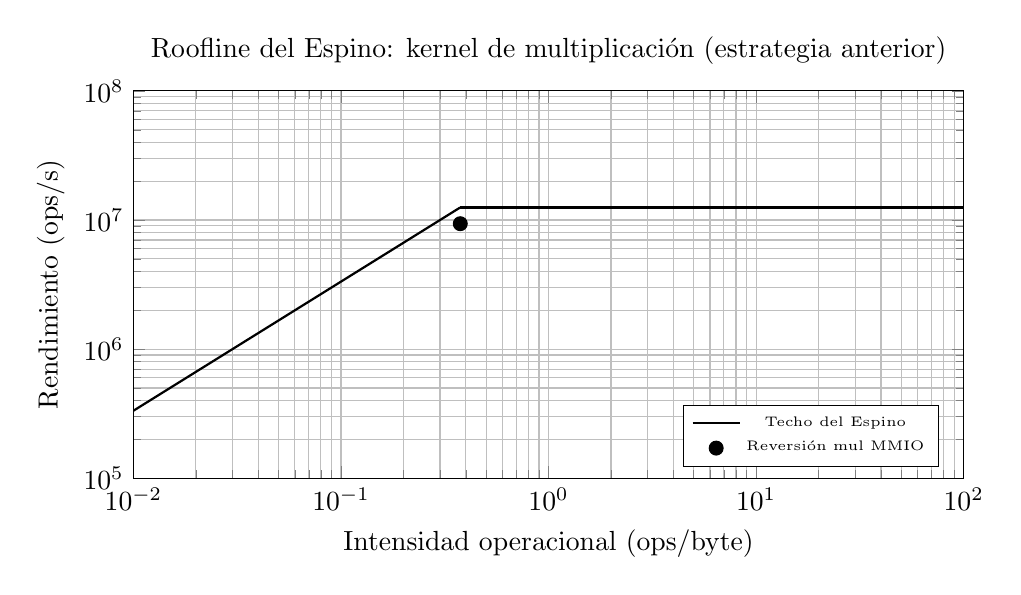
\begin{tikzpicture}
\begin{axis}[
  xmode=log, ymode=log,
  xlabel={Intensidad operacional (ops/byte)}, ylabel={Rendimiento (ops/s)},
  title={Roofline del Espino: kernel de multiplicación (estrategia anterior)}, legend pos=south east, legend style={font=\tiny},
  xmin=0.01, xmax=100, ymin=1e+05, ymax=1e+08, grid=both,
  width=\linewidth, height=6.5cm]
\addplot[thick, black, domain=0.01:0.375, samples=2] {3.33333e+07*x};
\addplot[thick, black, domain=0.375:100, samples=2, forget plot] {1.25e+07};
\addlegendentry{Techo del Espino}
\addplot[only marks, mark=*, mark size=2.5pt] coordinates {(0.375724,9.36598e+06)};
\addlegendentry{Reversión mul MMIO}
\end{axis}
\end{tikzpicture}
